\documentclass[12pt]{article}
\usepackage[utf8]{inputenc}
\usepackage{graphicx} % Allows you to insert figures
\usepackage{amsmath} % Allows you to do equations
\usepackage{fancyhdr} % Formats the header
\usepackage{geometry} % Formats the paper size, orientation, and margins
\usepackage{caption}
\usepackage{subcaption}
\usepackage[style=authoryear-ibid,backend=biber]{biblatex} % Allows you to do citations - does Harvard style and compatible with Zotero
\addbibresource{Example.bib} % Tells LaTeX where the citations are coming from. This is imported from Zotero
\usepackage[english]{babel}
\usepackage{csquotes}
\renewcommand*{\nameyeardelim}{\addcomma\space} % Adds comma in in-text citations
\linespread{1.25} % About 1.5 spacing in Word
\setlength{\parindent}{0pt} % No paragraph indents
\setlength{\parskip}{1em} % Paragraphs separated by one line
\renewcommand{\headrulewidth}{0pt} % Removes line in header
\geometry{a4paper, portrait, margin=0.7in}
\setlength{\headheight}{14.49998pt}
\usepackage{titlesec}
\titlespacing{\subsection}{1pt}{\parskip}{-\parskip}
\begin{document}
	\begin{titlepage}
		\begin{center}
			\vspace*{5cm}
			
			\Huge{Weekly Reports}
			
			\vspace{0.5cm}
			\LARGE{Mehmani Research Group}
			
			\vspace{3 cm}
			\Large{}
			
			\vspace{0.25cm}
			\large{Nicolás Bueno Zapata}
			
			\vspace{3 cm}
			\Large{Spring 2022}
			
			\vspace{0.25 cm}
			\Large{Pennsylvania State University}
			
			
			\vfill
		\end{center}
	\end{titlepage}
	
	\setcounter{page}{2}
	\pagestyle{fancy}
	\fancyhf{}
	\rhead{\thepage}
	\lhead{Nicolas's Reports}
	
	\section*{Jan 30, 2022}
	 During this week I was focoused on testing my LBM code for a single component and multiphase conditions. For validation, I looked for other available codes from the postdoc, Cheng, and codes available in the Dr. Ayala's research group. I had to redefine some objects in my code to be able to pursue the next modeling objectives as:
		
	\begin{itemize}
		\item Have different relaxation parameters for every component
		\item Have more than one force applying to our components 
		\item The components also have the propety "pseudopotential"

	\end{itemize}

	I was reading how to model two immiscible components through LBM, and I discover that the treatment of Cheng is quite different (valid, though) from the proposed in Kruger's book. I created a new routine with a different Shan-Chen force implementation (each component uses its own pseudopotential) for immiscible displacement, because I want to be able to simulate a case where I inject a single component that displaces the other, although I just realize that I need to specify the composition of my injecting fluid for all the boundary conditions we have specified. In single component, specifing the pressure is equivalent to specify the density. However, for multi-component, we need to provide the amount of each component at that pressure to be able to have a solvable system.
	
	I decided to keep track of all the different options and equations inside the code, and I started to write my own LBM document to explain to myself and future users, what are the equations implemented and the logic behind them. 
	
	It has been difficult to balance the time for research, coding, and reading papers where to inspire for research ideas and applications. I am still trying to find the correct point in this semester, as all the courses are kind of related to my thesis, and all deserve the same degree of attention. 
	
	\pagebreak
	
	\section*{Feb 6, 2022}
	
	\subsection*{Things that were done}
	This week started the full implementation of the multi-relaxation-times collision operator for my LBM model. Despite the first coding stage, I had programmed classes for collisionMRT operator and the lbmParameter object, these two were somehow in conflict, as the Fortran polymorphism is somehow more strict than in C++, so I had to arrange the code to account for generalization in the main routines, who do not know in principle, which type of object are they calling to. I read about LAPACK, a library to handle linear systems in Fortran, that could be useful for other problems and applications using the code in development. 
	
	Another advance in this matter was the two-phase flash algorithm that is almost working in C++. The purpose of this code is to have my own library for thermodynamic analysis of mixtures (solve stability, n-phase flash, envelopes, bubble points) that can give insights in how to set a simulation case for the LBM code. The novelity with this code is that is connected with Matplotlib, library from Python, so it can be used any plot command from there in C++. I would like to improve the Subsequent Substitution Method by a Newtonian algorithm using the C++ Library, Eigen, to solve linear systems of equations. 
		
	\subsection*{Difficulties}
	This semester, as particularly intense, has been difficult to balance between study and working times. However, I have managed to take advantage of the homework and classes to enforce my knowledge, especially that related with my field of research and expertise: thermodynamic behavior of mixtures, pore-scale phenomena, scientific-programming, and fluid-flow modeling. I also have come across challenges regarding the object-oriented programming with Fortran. There are plenty resources online, but hardly there is one canonical source as there is for C++. 
	
	\subsection*{Work for next week}
	I will validate the MRT collision operator with the Cheng's codes for single component. After this, I will validate for two components. If I reach this point, I will be able to write the paper that he left in progress, and I can focus on particular problems (applications) and the parallelization with OpenMPI. I will start selecting some papers to delimit the fields where this multiphase model could be applied, as I need to have a goal for the method, so I can take some decisions in advance. As capillary pressure is of our interest, it is worth asking if the 3D implementation is a priority in the research. 
	
	Ask for access to the report template.
	
	\pagebreak
	\section*{Feb 7 - Feb 12}
	\subsection*{What was done last week}
	This week I finished the coding of the multi-relaxation times (MRT) collision operator. As this operator implies the multiplication of matrices and vectors, I used the Fortran built-in operator for this purpose, although later on a manually multiplication can be coded to gain computational speed (that is not a priority right now, but I keep saving notes for future improvements). At this point, it is worth mentioning the simulations I am running make use of an cubic equation of state, that was validated months ago, before taking a detour to validate single phase problems with analytical solutions, that I presented before going to the Winter break. Now, the validation cases combine single or multi-component cases with BGK or MRT as the collision operator. The results of the previous BGK implementation show a successful match between my model and the Cheng's legacy code (Dr. Ayala's post-doc), for static and oscillating droplets of a single component/multiphase model. The MRT model was successfully implemented, and the static droplet case was validated (Figure \ref{fig:val1CMRT}). However, the case for the oscillating droplet has presented difficulties in terms of model interpretability, and results availability (see difficulties). During the week, I wanted to clarify some ideas that were taking me to different directions. As I am conscious about how important it is to focus on a single task, I tried to discriminate between interesting ideas to pursue later, and the important research aspects that have to be addressed from now. So, apart from coding, I made a preliminary review about current multiphase applications where LBM is a suitable model. I found an interesting topic, called self-propelled droplets, where acceleration is exerted by surface tension gradients caused by non-uniform fields of whether surfactant concentration or temperature. This search is obeying my believe on that concrete applications help to visualize and give shape to the current and future code, at the time it motivates me to be in current hot-spots for research (I want to be close to topics of high applicability). In that sense, I discovered the Marangoni-like flow, I found some papers simulating the phenomena with LBM, and I plan to read a couple during the week and possibly bringing them for the next group meeting.  
	
	\begin{figure*}[h]
		\centering
		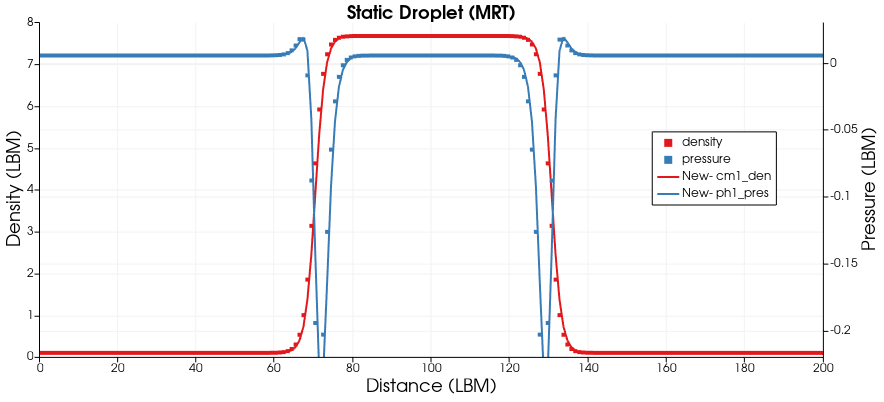
\includegraphics[scale=0.4]{pics/MRT_StaticDroplet_PRho.png}
		\caption{Comparison of pressure and density.}
		\label{fig:val1CMRT}
	\end{figure*}
	 
	\subsection*{What will be done next week?}
	I will finish the MRT validation against Cheng's codes, but this paradigm is becoming more complex every time, as the codes are extensive and each one changes its input parameters. I feel that attach to simpler but extensively reported cases would be better for our purpose. As the MRT code is already running and giving good results (qualitatively), I consider the two-component case is ready to be addressed. The code is already generalized, so the only missing part is to configure the cases and start running and debugging. 
	
	\subsection*{Difficulties}
	\begin{itemize}
		\item The MRT case does not show several oscillations as the BGK does. 

		\item The BGK has only one parameter that relates to the viscosity of the fluid, so I can control how fast the momentum diffuses through this parameter. However, MRT has more parameters, and sometimes they look like \textit{magic-parameters}, that I am still understanding to produce stable simulations.
		\item There are many validation codes, and handling that amount of versions is becoming overwhelming. How can I generate enough trust in the model?
		\item Side note: The phase behavior model I have in C++ started as a class project the last semester for the Advance Programming course, and is the mandatory project for the Thermodynamics course I am taking this semester. That is the reason I am developing the code, and the fact it is in C++ is because I want to improve my proficiency with high-performance programming languages. 
	\end{itemize}


	\pagebreak
	\section*{Feb 14 - Feb 19}
	\subsection*{What was done last week}
	According to the plan from past week, and given the instructions by Dr. Ayala, I ran again the oscillation droplet for BGK and MRT, and compared against my code. After a tough debugging process, I discovered the cause (difference in numerical parameters) of the discrepancies in the MRT case. Now, both codes are providing the same results for the two collision operators (figure \ref{fig:osci}). This debugging process lead me to repeat the Cheng's previous MRT implementation, that although is manual and cumbersome, accelerates considerable the code as no matrix-vector operations are needed. As a parallel example, I ran the case of a falling droplet, that marked the importance to generalize the viscosity as a value per phase.
	
	I skimmed through some papers studying the Marangoni flow with LBM solvers. Part of this search was presented in the Friday's meeting, where I could understand better (not completely) the phase-field model based on the free-energy functional. Although no research related, I consider important to inform that I sent the documentation to apply for a Minor in Computational Science, although last semester I took most of the credits needed for this goal, and only 6 credits are missing for this purpose, apart from the missing research credits I have pending. 
	
	\begin{figure}[h]
		\centering
		\begin{subfigure}{.5\textwidth}
			\centering
			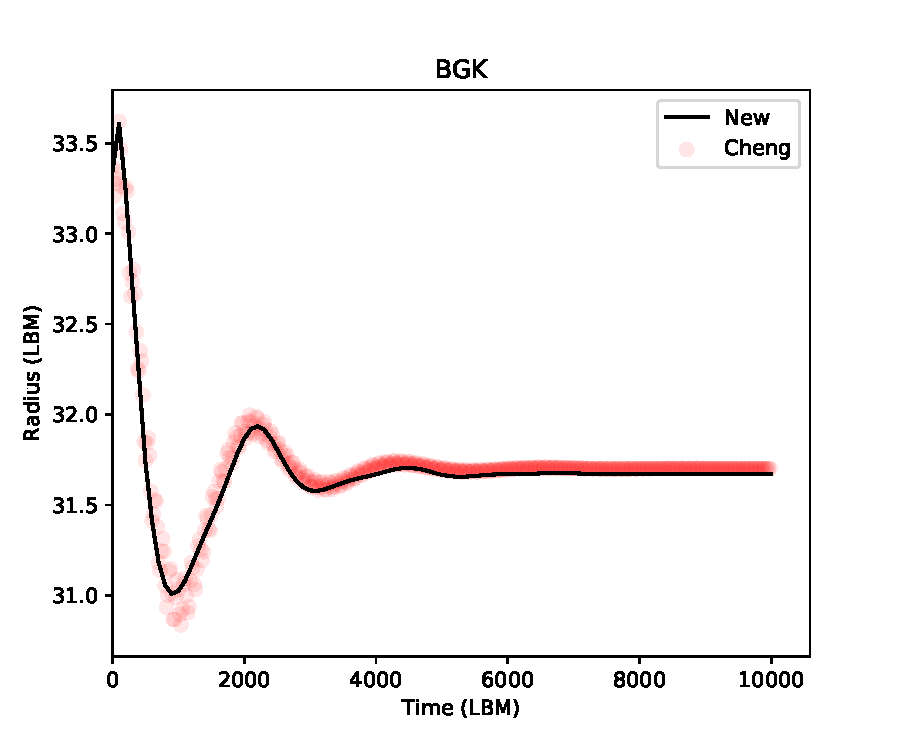
\includegraphics[width=.6\linewidth]{pics/BGKOsc.pdf}
			\caption{BGK}
			\label{fig:sub1}
		\end{subfigure}%
		\begin{subfigure}{.5\textwidth}
			\centering
			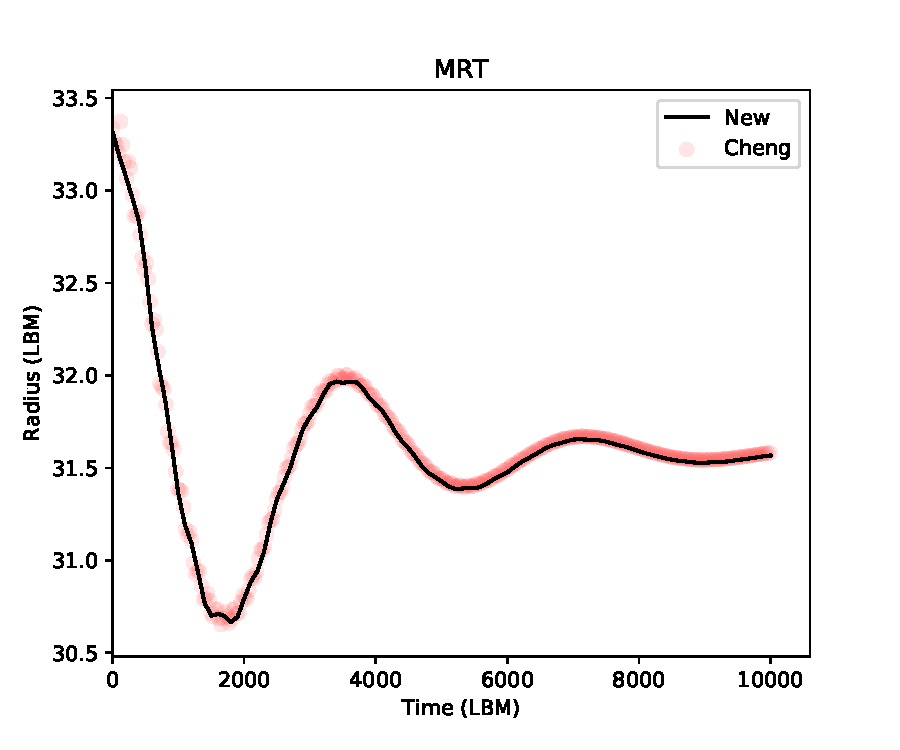
\includegraphics[width=.6\linewidth]{pics/MRTOsc.pdf}
			\caption{MRT}
			\label{fig:sub2}
		\end{subfigure}
		\caption{Oscillation droplet case. Viscosities are different in each case.}
		\label{fig:osci}
	\end{figure}
	
	\subsection*{Difficulties}
	\begin{itemize}
		\item One difficulty raised from the high terminal velocity that a falling droplet reaches due to gravity. I haven't had the time to test a rising bubble (may present a smaller velocity) but it would be a good match example once I fixed the viscosity per phase. In fact, I feel I have not understood the advantages that LBM can provide in terms of physics modeling, and I should be better aware of both its limitations and benefits, compared with the others well-known methods. 
		
		\item I also have had a debugging difficulty with GDB and Fortran, as sometimes the run simply collapse when I intend to access some object's information.
		
		\item I found myself confused with the management of information regarding my own advances and thoughts, and with migrating them from where I was accustom to (Discord, Obsidian).
	\end{itemize}
	 
	
	\subsection*{What will be done next week?}
	I forecast a busy week due to an exam I have on Thursday, the talk given by Dr. Pyrak, two homework for the next week, and a meeting with Dr. Ayala's research group, that includes Cheng as a guest to discuss the LBM difficulties. With the available time, I will start the 2-component case (oscillating droplet). I would like to receive some feedback during next weeks, about the direction we are going with the code and research objectives, maybe in a separate short-meeting between you Dr. Mehmani, and Dr. Ayala. During this week, the meeting with Cheng is particularly important, as there is where I can solve some concerns about LBM that are not clear enough in some books or papers, and where I can connect better with his ideas, and accelerate the paper writing. 
	


	%\pagebreak
	%\section*{Feb 7 - Feb 12}
	%\subsection*{What was done last week}
	%\subsection*{Difficulties}
	%\subsection*{What will be done next week?}
	\printbibliography % Be sure to remove access date and months from the .bib file
\end{document}